% Proposed solution: system architecture overview (issue #5; final report #63).
% Fig. system.png comes from docs/architecture/ (#18, updated in #76); re-exporting
% it there updates the report.

\section{Proposed Solution}
\subsection{Architecture Overview}
The accelerator computes products of signed $\mathrm{DATA\_W}$-bit fixed-point matrices. One run multiplies an $N \times k_{\mathrm{len}}$ block of $A$ by a $k_{\mathrm{len}} \times N$ block of $B$:
\begin{equation}
C[i][j] = \sum_{k=0}^{k_{\mathrm{len}}-1} A[i][k]\,B[k][j],
\label{eq:matmul}
\end{equation}
where the host chooses the inner length $k_{\mathrm{len}}$ for each run, from 1 to $K_{\max}$. A run can also \emph{accumulate}, adding its products onto the result of the previous run instead of starting from zero. With these two features the host can multiply matrices of any size, one $N \times N$ tile of $C$ and one chunk of the inner dimension at a time (Section~III-E). Table~\ref{tab:params} lists the parameters. Every module takes them as Verilog parameters, so the array size, the operand storage and the data widths change in one place.

\begin{table}[t]
\centering
\caption{Design parameters}
\label{tab:params}
\footnotesize
\begin{tabular}{@{}llc@{}}
\toprule
Parameter & Meaning & Default \\
\midrule
$N$ & array size; $C$ is computed in $N \times N$ tiles & 4 \\
$K_{\max}$ & largest inner length of one run & 16 \\
$\mathrm{DATA\_W}$ & operand width, signed & 8 \\
$\mathrm{ACC\_W}$ & accumulator and result width, signed & 32 \\
$\mathrm{FRAC\_W}$ & fractional bits of the Q-format reading & 0 \\
\midrule
$k_{\mathrm{len}}$ & inner length of a run, set by the host & 1 to 16 \\
$T$ & compute cycles of a run, $k_{\mathrm{len}} + 2N - 2$ & 7 to 22 \\
\bottomrule
\end{tabular}
\end{table}

\begin{figure*}[t]
\centering
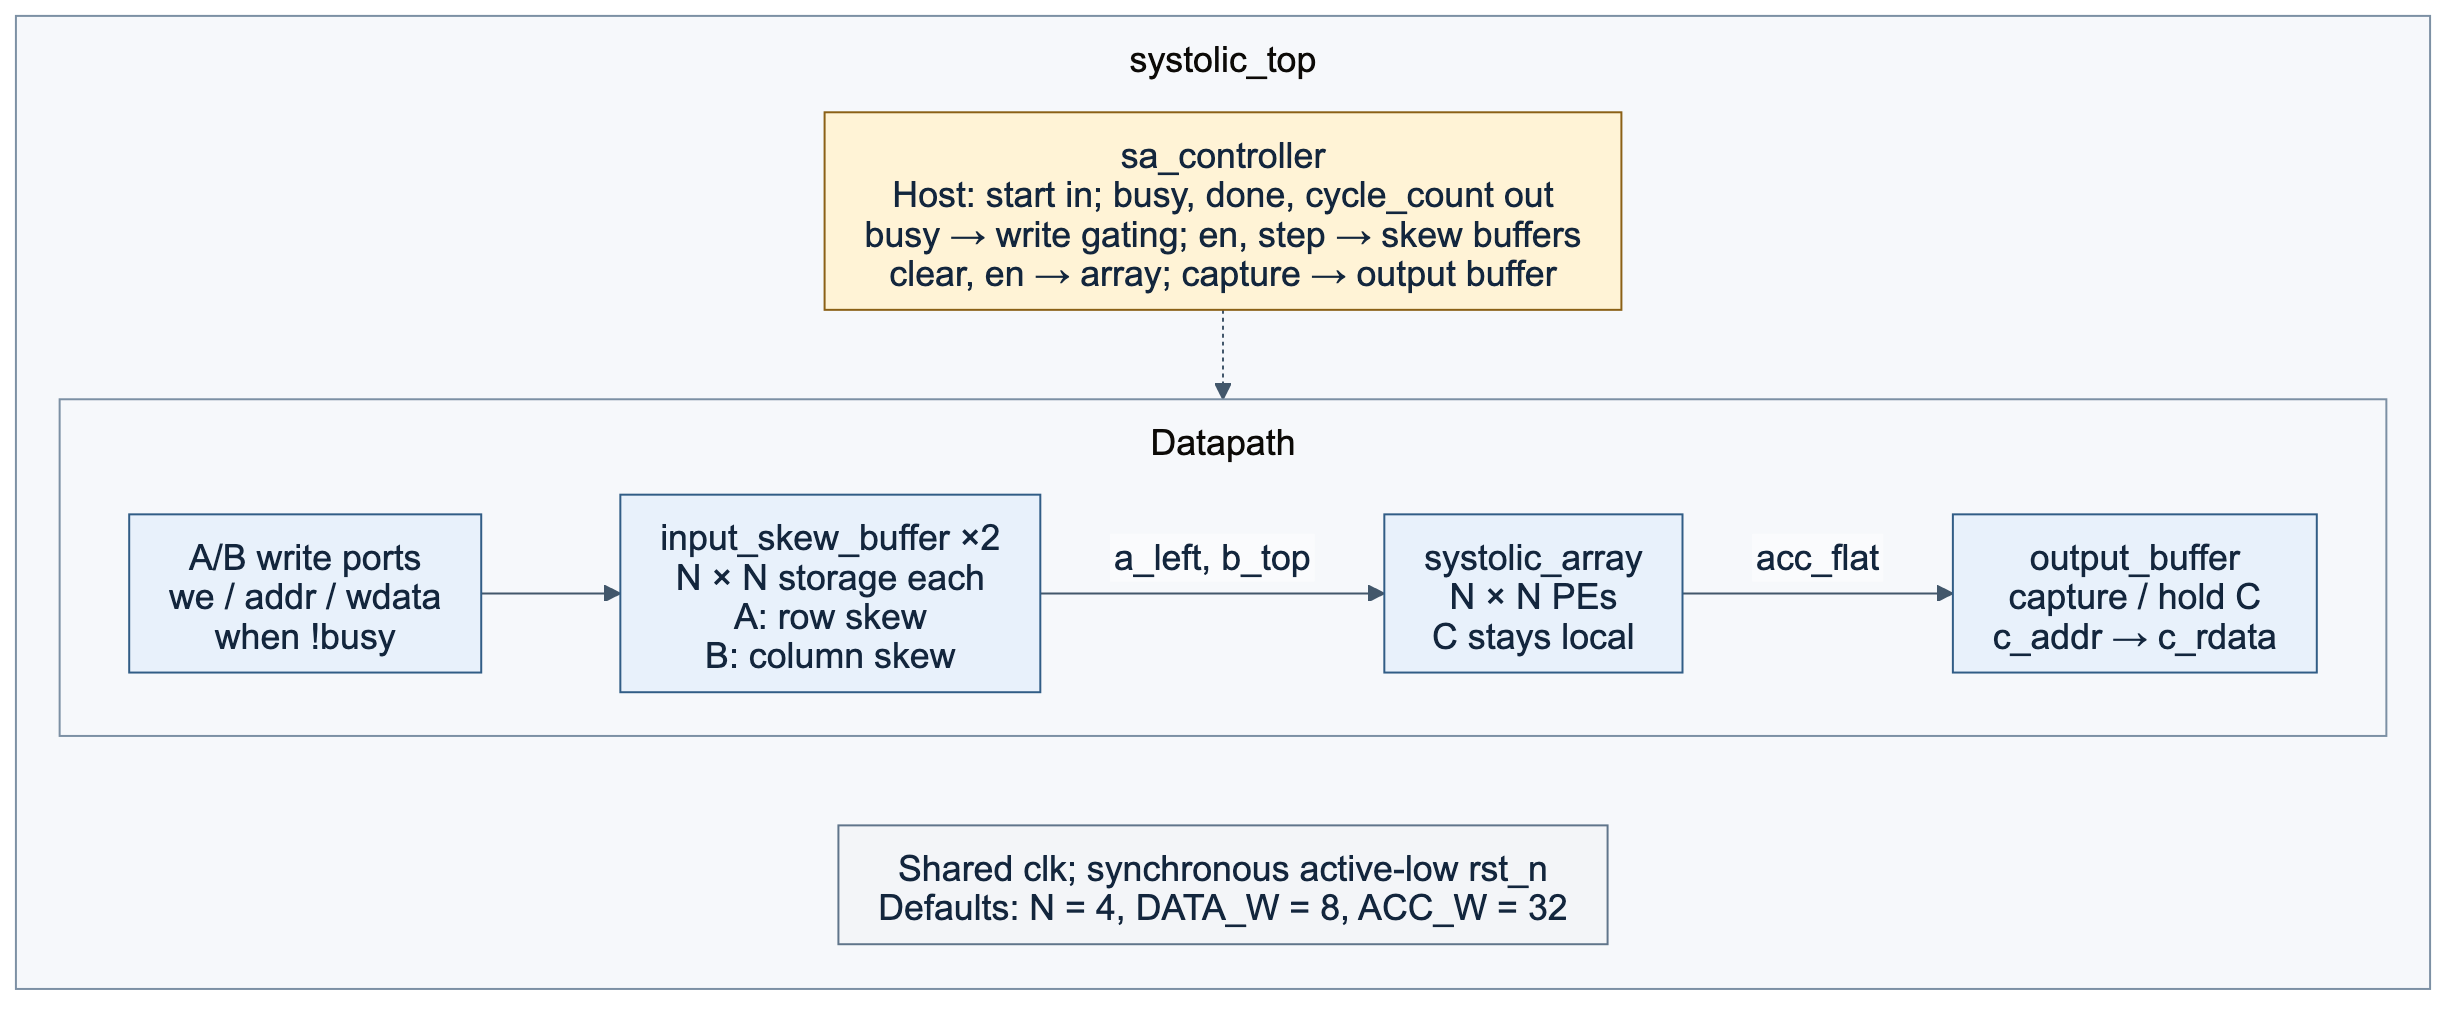
\includegraphics[width=\textwidth]{system.png}
\caption{System architecture. Solid arrows carry data and dashed arrows carry controller signals. Host writes reach the input skew buffers only while \texttt{busy} is low. Each buffer stores one operand block and selects its skewed lanes from the compute step and the run's inner length. The controller samples $k_{\mathrm{len}}$ and \texttt{accumulate} with \texttt{start}, clears the array unless the run accumulates, enables it for $T$ steps and then captures the accumulators into the output buffer, which serves the read port.}
\label{fig:system}
\end{figure*}

The design has five blocks behind one host interface, shown in Fig.~\ref{fig:system}:
\begin{itemize}
\item \textbf{Two input skew buffers.} The A buffer stores $N$ rows of $K_{\max}$ elements and the B buffer $K_{\max}$ rows of $N$ elements. During a run, the A buffer drives element $k$ of row $i$ into the left edge in step $i + k$, and the B buffer drives element $k$ of column $j$ into the top edge in step $j + k$, for every $k < k_{\mathrm{len}}$. Elements beyond $k_{\mathrm{len}}$ are never sent, so old data in the buffers needs no clearing.
\item \textbf{The systolic array.} An $N \times N$ grid of PEs. PE $(i,j)$ multiplies the operands that reach it, adds the product to its accumulator, which holds $C[i][j]$, and passes $A$ to the right and $B$ down one cycle later. The array is the same as in Phase~1: the inner length only changes how long operands keep arriving. The PE is described in Section~III-B and the skew in Section~III-C.
\item \textbf{The output buffer.} Copies all $N^2$ accumulators in one cycle when a run ends, and serves them to the host through a read port. The previous result therefore stays readable while the next run computes.
\item \textbf{The controller.} A five-state machine that samples $k_{\mathrm{len}}$ and \texttt{accumulate}, clears the array unless the run accumulates, runs the $T$ compute steps, and signals the capture and the end of the run (Section~III-D).
\end{itemize}

The host sees a small matrix data interface. It writes $A$ and $B$ one element at a time through two write ports, $A[r][k]$ at address $rK_{\max} + k$ and $B[k][c]$ at address $kN + c$, sets $k_{\mathrm{len}}$ and \texttt{accumulate}, pulses \texttt{start}, waits for \texttt{done}, and reads $C$ one element at a time through the read port. A \texttt{start} whose $k_{\mathrm{len}}$ is 0 or above $K_{\max}$ is ignored, and \texttt{busy} stays low, so the host can see that it was rejected. While \texttt{busy} is high, writes are ignored, so the operands of a running product cannot change. Between runs $A$ and $B$ keep their contents, so a host can replace one operand and start again. A \texttt{cycle\_count} output reports how many cycles the last run took, which the testbenches use to check the latency.

A normal run spends one cycle clearing every accumulator and forwarding register, then $T = k_{\mathrm{len}} + 2N - 2$ compute steps in which the skewed operands cross the array and every PE adds its $k_{\mathrm{len}}$ products, and one more cycle copying the accumulators into the output buffer before \texttt{done} rises. \texttt{busy} is therefore high for $k_{\mathrm{len}} + 2N$ cycles: 12 for $k_{\mathrm{len}} = 4$ and 24 for $k_{\mathrm{len}} = K_{\max} = 16$. An accumulate run skips the clear and takes one cycle fewer.

The sequential baseline that the results compare against, \texttt{seq\_matmul}, has exactly the same ports and address map, so the same testbenches and the live demonstration drive both designs. It contains one multiplier and one adder with the same arithmetic as the PE, computes $C$ one element at a time, and is busy for $N^2 k_{\mathrm{len}}$ cycles per run.

The array performs $N^2 = 16$ MACs per cycle at its peak. A run performs $N^2 k_{\mathrm{len}}$ MACs in $T$ compute cycles, against $N^2 k_{\mathrm{len}}$ cycles for the baseline, a compute speed-up of $N^2 k_{\mathrm{len}}/T$: 6.4 for $k_{\mathrm{len}} = 4$ and 11.6 for $k_{\mathrm{len}} = 16$. Each PE is busy for $k_{\mathrm{len}}$ of the $T$ cycles, so utilization rises from 40\,\% at $k_{\mathrm{len}} = 4$ to 72.7\,\% at $k_{\mathrm{len}} = 16$, because the wavefront's $2N - 2$ cycles of fill and drain are paid once per run. Loading a run's operands through the one-element ports takes $N k_{\mathrm{len}}$ cycles, more than the run itself, so end to end the ports, not the array, limit throughput (Section~V).

The arithmetic is exact integer arithmetic. The 32-bit accumulators cannot overflow for any inner dimension below 131{,}072, counted across all the chunks of a tiled product (Section~III-B), so the datapath needs no rounding or saturation. Operands can also be read as Q-format fixed-point numbers with $\mathrm{FRAC\_W}$ fractional bits, and each element of $C$ then has $2\,\mathrm{FRAC\_W}$ fractional bits. This changes only how the numbers are read, not the hardware.
